\subsection{Shared covariance, fitting sensitivity and retuned data efficiency}
A subsequent exploratory track retains the full technical residual covariance across development pairs. Sixteen joint cell-bootstrap draws reuse shared single and control samples, and their residual covariance is averaged over the frozen output genes. The likelihood uses only each fitting fold's covariance block. Generalized least squares retains an unpenalized shared intercept; inner folds choose variance strength and off-diagonal shrinkage. The unweighted, diagonal and correlated searches contain 67, 201 and 469 candidates respectively. A jointly permuted training covariance has the same 469-candidate budget as the correlated family. No query responses enter these studies.

\begin{table}[htbp]\centering\small\resizebox{\linewidth}{!}{\begin{tabular}{llrrr}\toprule
Dataset & Split & Diagonal & Correlated & Permuted \\ \midrule
Norman & random & 1.26 to 1.48 & 0.97 to 1.47 & -0.20 to 0.00 \\
Norman & partner & 0.86 to 1.29 & 0.77 to 1.30 & 0.00 to 0.15 \\
Wessels original & random & 0.36 to 1.30 & 0.36 to 1.06 & -0.03 to 0.00 \\
Wessels original & partner & -0.42 to -0.07 & -0.42 to -0.07 & -0.03 to 0.02 \\
Wessels protected & random & -0.06 to 0.90 & 0.29 to 0.90 & -0.04 to 0.02 \\
Wessels protected & partner & -0.39 to -0.16 & -0.96 to -0.28 & -0.00 to 0.00 \\
\bottomrule\end{tabular}
}\caption{Percentage MSE reduction relative to the unweighted kernel over three additional development split seeds. Ranges are extrema of dependent resamplings, not confidence intervals. Negative reductions indicate worse error.}\end{table}

The correlated family improves Norman random error by 0.97--1.47\%, while diagonal weighting improves it by 1.26--1.48\%. Original Wessels random gains are 0.36--1.06\% for correlated noise and 0.36--1.30\% for diagonal noise. Both families worsen original and protected Wessels partner aggregates in these three seeds. Correlated protected random gains are 0.29--0.90\%. Thus the extra covariance parameters do not establish a consistent gain over the diagonal likelihood, and the additional split histories expose sensitivity in earlier positive findings.

For every correlated outer fit, each of the sixteen technical reference draws recomputes the reference-derived kernel and refits response coefficients. Predictions are scored against the point-estimated outer validation response. Recorded 5th, 50th and 95th error percentiles and gene-level prediction standard deviations quantify fitting/reference sensitivity conditional on the selected configuration, covariance, QC and normalizer. They do not include selection uncertainty or biological replication and are not confidence intervals for population performance.

Training subsets of one-quarter, one-half, three-quarters and full outer training size independently retune each kernel family using fitting-only inner folds. Three nested subset orders share the same outer validation set; full size is fitted once. Infeasible inner partitions are retained without response-dependent redraws. A fixed-full-size-hyperparameter kernel provides a comparator. A first curve run reordered the full-size pair list, changing its inner partition; it is retained. The corrected run uses canonical full-size order, and verifies identical fixed and retuned unweighted full-size predictions. Larger subsets improve error in these runs, while retuning itself has mixed effects. No independent sample-efficiency advantage follows from the correlated covariance extension.

\begin{figure}[htbp]\centering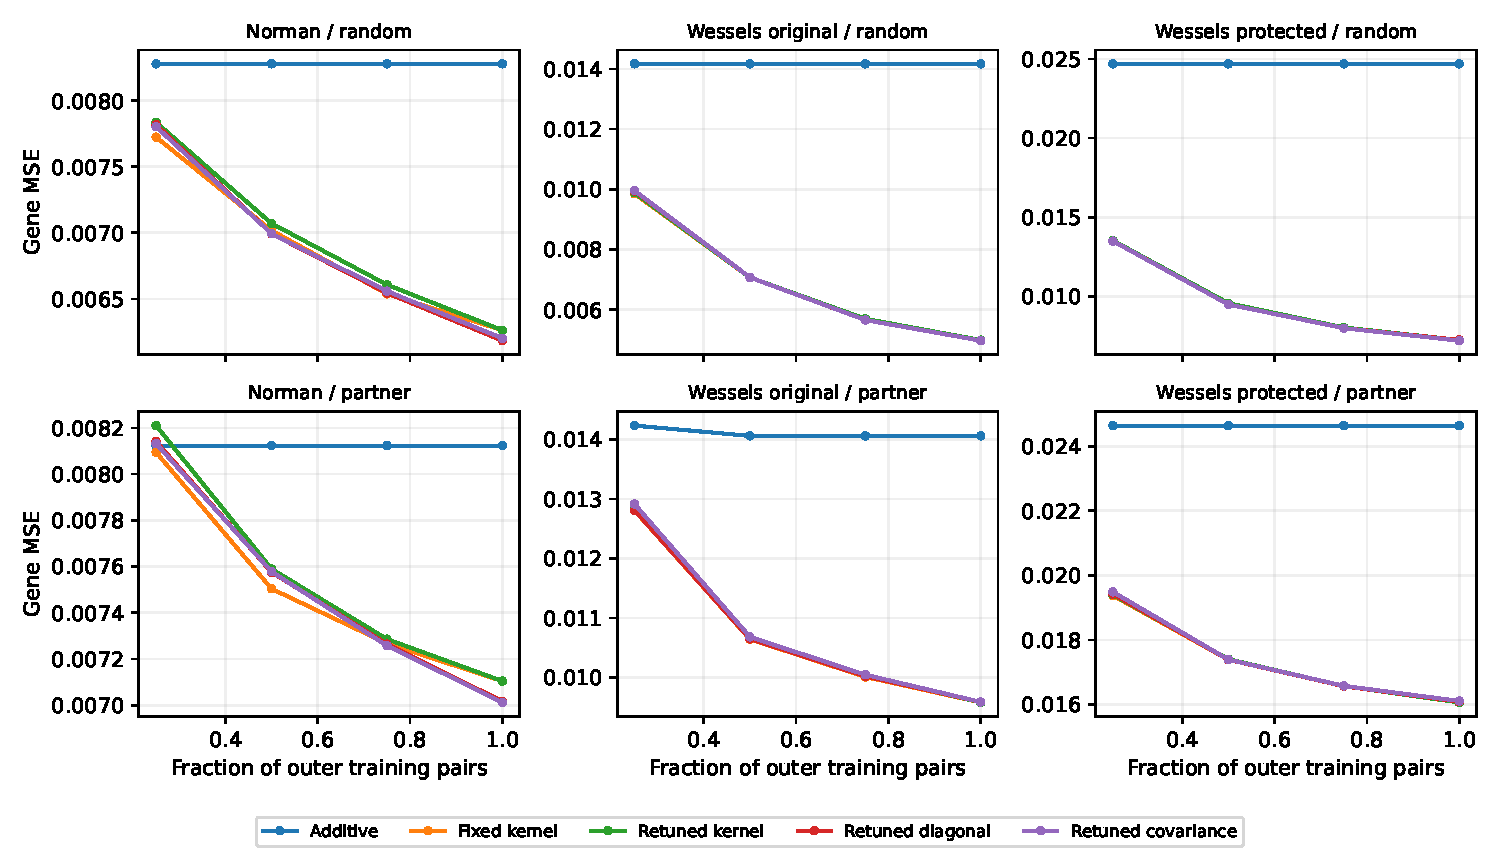
\includegraphics[width=\linewidth]{evidence/ceiling-learning-curves.pdf}\caption{Subset-retuned development learning curves with a fixed-hyperparameter kernel comparator. Subset orders and partner validation occurrences are dependent. Infeasible small-subset fits can change the scored occurrence population.}\end{figure}

A separate diagnostic divides each outer fitting population into fitting and calibration pairs. Only fitting responses select hyperparameters and fit the diagonal kernel. A condition-level gene-RMSE radius uses the finite-sample rank $\lceil(n+1)c\rceil$ for requested coverage $c$; ranks above the calibration sample count have no finite radius. Conformal coverage statements require appropriate exchangeability assumptions \citep{shafer2008}; these dependent biological pairs do not establish them. We report empirical outer coverage without implementing a calibrated abstention policy.

\begin{table}[htbp]\centering\small\resizebox{\linewidth}{!}{\begin{tabular}{llrrrr}\toprule
Dataset & Split & Nominal & Finite folds & Observed & Mean radius \\ \midrule
Norman & random & 80 & 5/5 & 81.8 & 0.0982 \\
Norman & random & 90 & 5/5 & 94.3 & 0.1270 \\
Norman & partner & 80 & 5/5 & 87.0 & 0.1195 \\
Norman & partner & 90 & 5/5 & 94.4 & 0.1333 \\
Wessels original & random & 80 & 5/5 & 85.0 & 0.1005 \\
Wessels original & random & 90 & 0/5 & -- & -- \\
Wessels original & partner & 80 & 5/5 & 71.8 & 0.1105 \\
Wessels original & partner & 90 & 4/5 & 84.7 & 0.1239 \\
Wessels protected & random & 80 & 5/5 & 76.4 & 0.1023 \\
Wessels protected & random & 90 & 5/5 & 90.0 & 0.1374 \\
Wessels protected & partner & 80 & 5/5 & 76.7 & 0.1604 \\
Wessels protected & partner & 90 & 5/5 & 83.7 & 0.1708 \\
\bottomrule\end{tabular}
}\caption{Isolated error-radius diagnostic on one development split seed. Nominal and observed coverages are percentages; mean radii are gene-RMSE units. Observed coverage counts only folds with finite radii and is descriptive.}\end{table}

Original Wessels random folds have seven calibration pairs, so a nominal 90\% finite radius is unavailable on every fold. Protected Wessels partner folds attain only 83.7\% empirical coverage at nominal 90\%, and original Wessels partner folds attain 84.7\% over their four finite-radius folds. These results do not support a usable guaranteed-risk release. The common \texttt{main.py ceiling} route reproduces this extension, and \texttt{main.py frontier} includes it in the full architecture build.
